\clearpage
\chapter{Qualitätssicherung mittels JUnit-Tests}

Zunächst wurde die Funktionalität der Methoden der Unternehmenssimulation anhand einfacher Konsolenausgaben durch die Entwickler unseres Teams getestet. Diese Art der Tests kann als Entwicklertest eingestuft werden. Die Entwicklertests werden in der Regel vom Entwickler selbst durchgeführt und dienen zur Überprüfung von Zwischenergebnissen und einzelnen Codezeilen. In dem untenstehendem Beispiel für einen Entwicklertest ist zu sehen, wie die Methoden getAktuellerSpieler() und naechsterSpieler() durch einfache Konsolenausgaben überprüft wurden.

\lstset{language=Java}
\begin{lstlisting}
	// Naechster Spieler ist dran 
	System.out.println("Spieler " + spiel.getAktuellerSpieler() + " am Zug");
	System.out.println("Naechster Spieler!");
	spiel.naechsterSpieler()	
	System.out.println("Spieler " + spiel.getAktuellerSpieler() + " am Zug")	System.out.println();
\end{lstlisting}

Nachdem die Funktionalität der Methoden überprüft und gegebenenfalls angepasst wurde, konnte mit dem Schreiben von JUnit-Tests begonnen werden. Unit-Tests, auch Modultests genannt, überprüfen einzelne isolierte Komponenten wie beispielsweise Methoden. Dadurch ist es möglich, Fehler schnell und einfach zu erkennen. Eine Änderung muss oft nur an einer Stelle vorgenommen werden, da die Methoden unabhängig voneinander sein sollen. Da in unserem Projekt viele Methoden aufeinander aufbauen, war es nicht möglich, alle Methoden isoliert zu testen. Es existiert jedoch immer ein Test, der zunächst die Grundlage testet, zum Beispiel einen Spieler zu erstellen. Diese Methode wird dann in nachfolgenden Tests erneut aufgerufen, um eine logische Einheit abbilden zu können. Das Testen einer sinnvollen Einheit ist uns wichtiger, als ein isoliertes Detail zu testen, welches aber in dieser Form kein Mehrwert bringt.

\lstset{language=Java}
\begin{lstlisting}
	public void erstelleSpielerTest() {
		Spielbrett spielbrett = new Spielbrett(10, 10000, 0.1);
		Unternehmen[] spieler;
		
		spielbrett.erstelleSpieler(2);
		spieler = spielbrett.getSpieler();
		
		assertEquals("Spieler wurde nicht korrekt erstellt", 2, spieler.length);
	}
\end{lstlisting}

In dem obigen Beispiel ist ein JUnit-Test unserer Unternehmenssimulation zu sehen. Dieser Test überprüft die Erstellung der Spieler.

Um einen Spielablauf simulieren zu können, wurde ein Szenariotest geschrieben. Anders als beim Unit-Test prüft dieser das Zusammenspiel der einzelnen Methoden, wodurch ein Programmablauf nachgeahmt werden kann. Der Szenariotest überprüft somit auch die Eingaben, die ein Nutzer auf der Benutzeroberfläche vornehmen kann.
Der Szenariotest besteht aus drei Runden, damit ausreichend Funktionalität abgedeckt werden kann. 
\\
In der ersten Runde werden drei Spieler in den jeweils drei unterschiedlichen Marktsegmenten erstellt. Jeder Spieler erforscht in seinem Segment eine Uhr, die dann produziert wird. \par
In der zweiten Runde können die produzierten Uhren am Markt angeboten werden. Jeder Spieler entwickelt zusätzlich in seinem Segment einen Bestandteil der Uhr (Armband, Gehäuse und Uhrwerk). Des Weiteren wird der Einkauf erweitert, wodurch die Selbstkosten gesenkt werden können. Anschließend wird nochmals produziert. 
In der dritten Runde werden erneut die produzierten Uhren angeboten. Die Produktion wird erweitert, wodurch das Produktionslimit gesteigert wird und somit mehr Uhren produziert werden können. Die letzten Funktionen, die der Szenariotest abbildet, sind die beiden Marketingstrategien. Diese setzen sich aus dem Uhrenmarketing, welches ein einzelnes Uhrenmodell bewirbt und dem Unternehmensmarketing, welches das Unternehmen als Ganzes betrifft, zusammen. 
Abgeschlossen wird der Test durch die Ermittlung des Siegers mittels einer assertEquals-Abfrage. Die genaue Platzierung der restlichen Spieler bleibt hierbei jedoch unberücksichtigt, da die Methode, welche die Platzierung der Gewinner ermittelt, privat ist, damit die Gewinnermittlung nicht von außen beeinflussbar ist. 

\begin{figure}[!h]
	\centering
	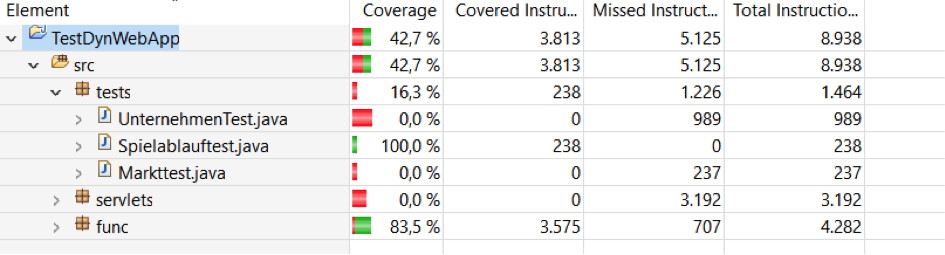
\includegraphics[scale=0.8]{img/bild1_tests.png} 
	\caption{Coverage des Szenariotests} \label{fig:abb31}
\end{figure}

Dem Screenshot ist zu entnehmen, dass der Szenariotest „Spielablauftest“ unsere Unternehmenssimulation zu 42,7\% abdeckt. 

Die JUnit-Tests unserer Unternehmenssimulation wurden in drei Testklassen aufgeteilt, um die Tests übersichtlicher zu gestalten. Somit testest z.B. der Markttest Methoden des Markts, welche jedoch teilweise Methoden des Unternehmens voraussetzen. Daher wurden manche Methoden sowohl im Unternehmenstest als auch im Markttest durchgeführt. Die drei Testklassen erreichen zusammen eine Codecoverage von 61,1\%. In dem Screenshot ist zu erkennen, dass alle Klassen des Pakets „func“ zu mindestens 80\% getestet wurden. Die Codecoverage wurde durch das Auslassen des Tests für das Servlet verringert. 

\begin{figure}[!h]
	\centering
	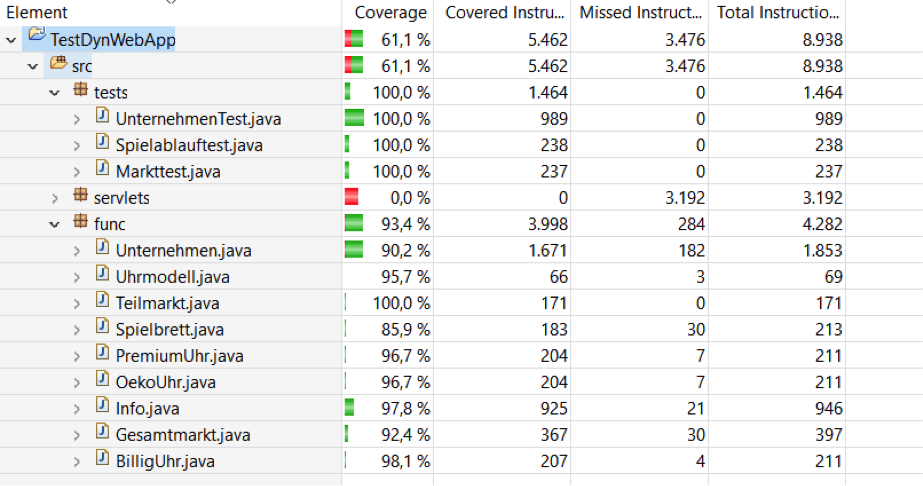
\includegraphics[scale=0.8]{img/bild2_tests.png} 
	\caption{Gesamte Coverage} \label{fig:abb32}
\end{figure}

Beim Ausgrenzen des Servlets von der Codecoverage wird die Unternehmenssimulation zu 95,1\% durch Tests abgedeckt. 

\begin{figure}[!h]
	\centering
	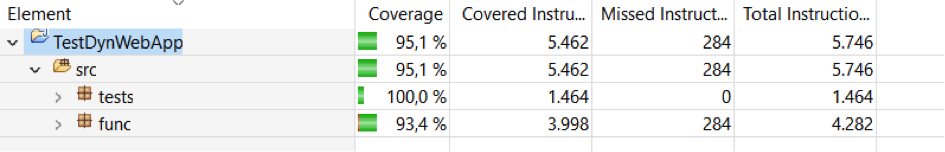
\includegraphics[scale=0.8]{img/bild3_tests.png} 
	\caption{Gesamte Coverage (ohne Servlets)} \label{fig:abb33}
\end{figure}







